\section{Preparations and calibration of the setup}

\begin{figure}[htbp]
    \centering
    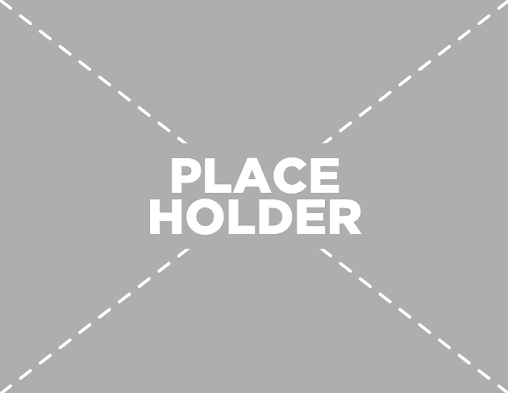
\includegraphics[width=0.5\linewidth]{Figures/Placeholder.png}
    \caption{Circuit diagrams}
    \label{fig:circuitdiagrams}
\end{figure}


\subsection{Gain of the amplifiers}

\begin{figure}[htbp]
    \centering
    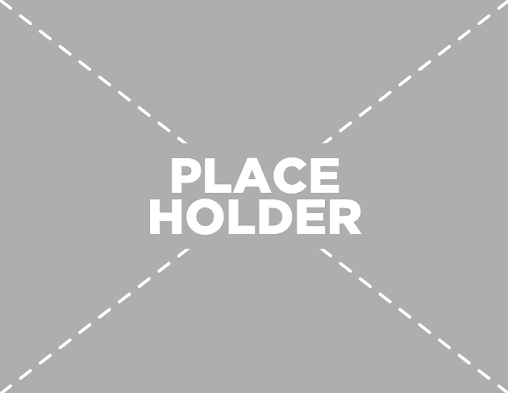
\includegraphics[width=0.5\linewidth]{Figures/Placeholder.png}
    \caption{Oscilloscope screenshot for both detectors}
    \label{fig:OscAmpGain}
\end{figure}

\subsection{Calibration of the SCAs}

\begin{figure}[htbp]
    \centering
    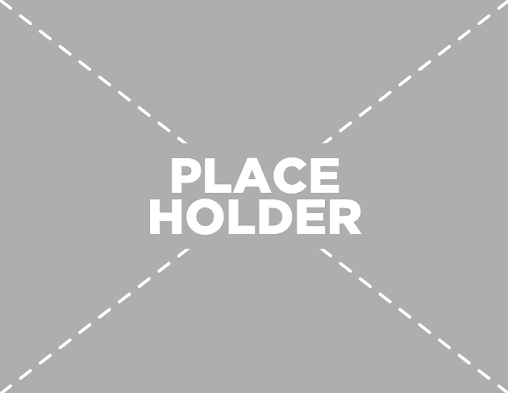
\includegraphics[width=0.5\linewidth]{Figures/Placeholder.png}
    \caption{MCA spectrum with and without SCA gate}
    \label{fig:MCA_SCA}
\end{figure}

\begin{equation}\label{eq:sensitivitySCA}
    AAAA = BBB
\end{equation}

\begin{figure}[htbp]
    \centering
    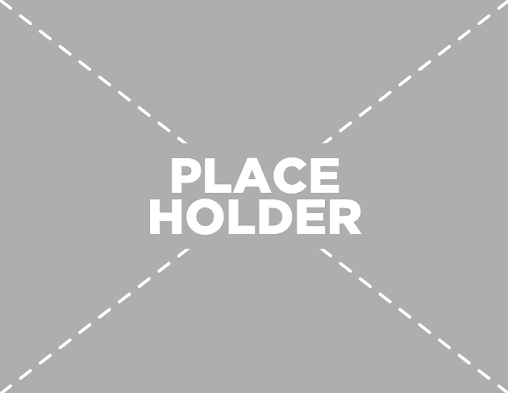
\includegraphics[width=0.5\linewidth]{Figures/Placeholder.png}
    \caption{Sensitivity of both detectors}
    \label{fig:Sensitivity}
\end{figure}

\subsection{Calibration of the CFDs}

\begin{figure}[htbp]
    \centering
    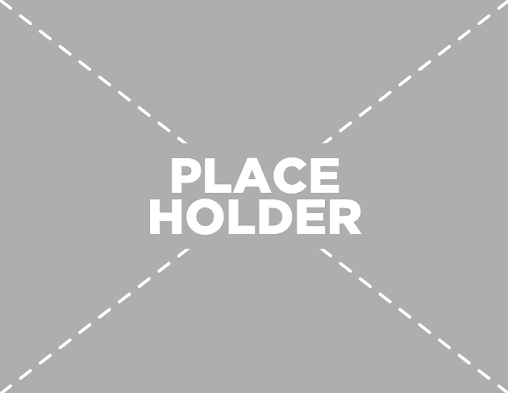
\includegraphics[width=0.5\linewidth]{Figures/Placeholder.png}
    \caption{MCA spectrum with and without CFD gate}
    \label{fig:MCA_CFD}
\end{figure}

\begin{equation}\label{eq:sensitivityCFD}
    AAAA = BBB
\end{equation}

\begin{figure}[htbp]
    \centering
    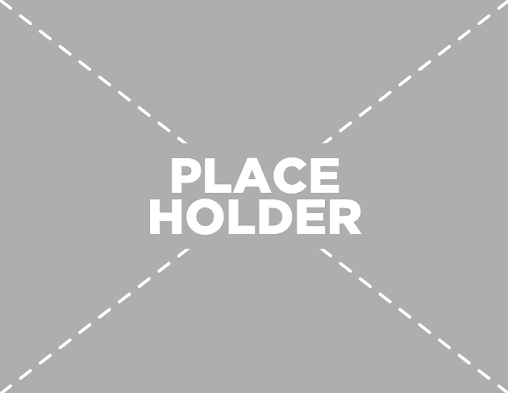
\includegraphics[width=0.5\linewidth]{Figures/Placeholder.png}
    \caption{Sensitivity of both detectors}
    \label{fig:SensitivityCFD}
\end{figure}

\subsection{Delay in the fast branch}

\begin{equation}\label{eq:Delay_Fast_Branch}
    CAD =asas
\end{equation}

\begin{figure}[htbp]
    \centering
    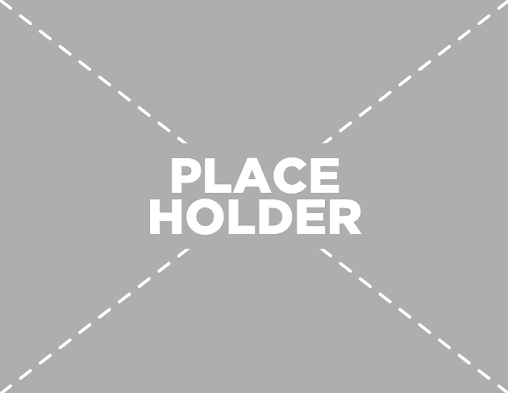
\includegraphics[width=0.5\linewidth]{Figures/Placeholder.png}
    \caption{Data delay fast branch with fit}
    \label{fig:Delay_data_raw}
\end{figure}

\begin{tabular}{c|c}
    a & b \\
    c & a
\caption{Fit parameters for the delay in the fast branch}
\label{tab:fit_delay_fast_branch}
\end{tabular}

\subsection{Delay in the slow branch}

\begin{figure}[htbp]
    \centering
    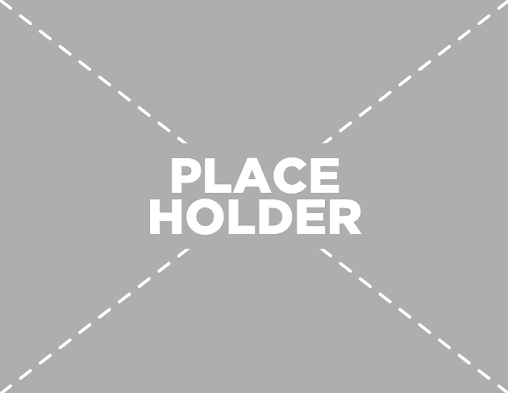
\includegraphics[width=0.5\linewidth]{Figures/Placeholder.png}
    \caption{Oscilloscope signal for the 3 branches}
    \label{fig:slow_delay}
\end{figure}

\FloatBarrier

\section{Main Measurement}

\subsection{Stability of the setup}

\begin{figure}[htbp]
    \centering
    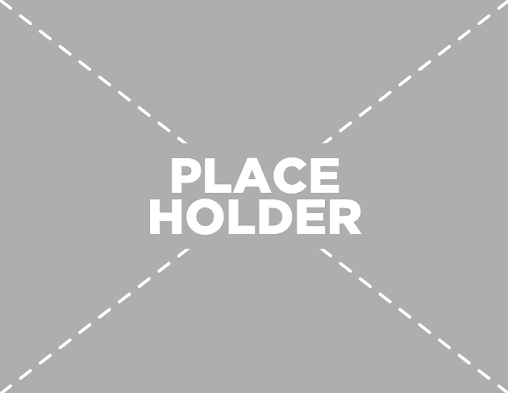
\includegraphics[width=0.5\linewidth]{Figures/Placeholder.png}
    \caption{Stability plot for both detectors.}
    \label{fig:stability_both}
\end{figure}

\begin{figure}[htbp]
    \centering
    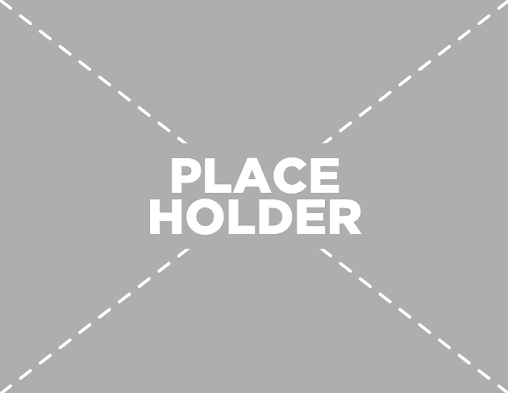
\includegraphics[width=0.5\linewidth]{Figures/Placeholder.png}
    \caption{Stability for the fast and universal coincidences}
    \label{fig:placeholder}
\end{figure}

\begin{tabular}{c|c}
    a & b \\
    c & d
\caption{Fit parameters for the stability}
\label{tab:fit_stability}
\end{tabular}

\subsection{Random coincidence and misalignment corrections}

\begin{table}[htbp]
    \centering
    \caption{Misalignment correction factor per angle}
    \label{tab:correction_factors}
    \begin{tabular}{c|c}
        a & b \\
        c & d
    \end{tabular}
\end{table}

\begin{figure}[htbp]
    \centering
    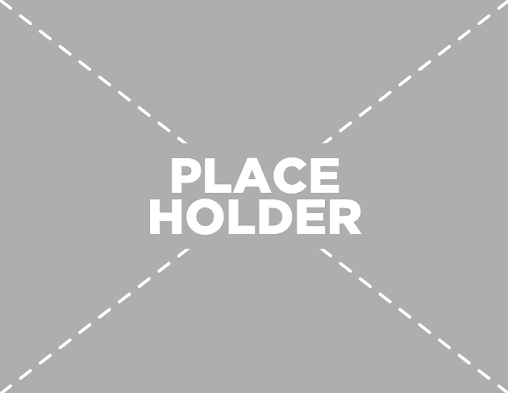
\includegraphics[width=0.5\linewidth]{Figures/Placeholder.png}
    \caption{Angular correlation after random coincidence and misalignment corrections}
    \label{fig:Angular_correl}
\end{figure}

\subsection{Measurement of the angular correlation}

\begin{equation}\label{eq:angular_correlation}
    CCCC = DDD
\end{equation}

\begin{figure}[htbp]
    \centering
    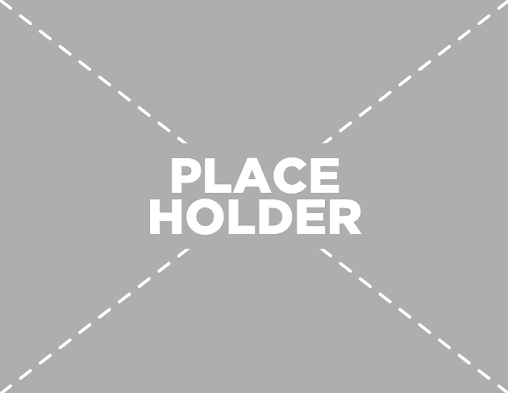
\includegraphics[width=0.5\linewidth]{Figures/Placeholder.png}
    \caption{Corrected count rates vs angle}
    \label{fig:Count_rates}
\end{figure}

\begin{table}[htbp]
    \centering
    \caption{Fit parameters of the angular correlation}
    \label{tab:fit_angular_correlation}
    \begin{tabular}{c|c}
        a & b \\
        c & d
    \end{tabular}
\end{table}

\begin{figure}[htbp]
    \centering
    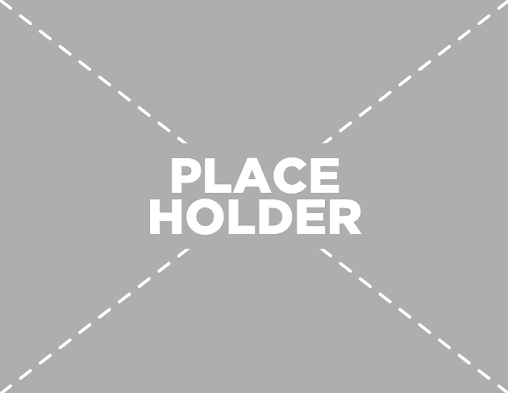
\includegraphics[width=0.5\linewidth]{Figures/Placeholder.png}
    \caption{Fit for cascade for different spins}
    \label{fig:Fits_cascades}
\end{figure}

\begin{table}[htbp]
    \centering
    \caption{Fit parameters for the different spin cascades}
    \label{tab:fit_spin_cascades}
    \begin{tabular}{c|c}
        a & b \\
        c & d
    \end{tabular}
\end{table}

\FloatBarrier

\section{Results and discussion}